\chapter{Algoritmul de recomandare }
\label{chap:ch1}

\section{Prelucrarea datelor}
\label{sec:ch3sec1}
\par Un prim pas în algoritmul de recomandare de filme este de a prelucra datele pentru a obține cele mai bune valori în calculul final al scorului. După ce avem toate datele primul pas este să înlocuim datele nule cu caracterul spațiu pentru a nu conta în calculul final. Apoi un pas destul de important în procesarea datelor este să eliminăm cuvintele de legătură ca de exmplu: ‘an’, ‘be’, ‘some’, etc. Cel mai important câmp din care trebuie scoase aceste cuvinte este descrierea deoarece la final se vor crea vectori din cuvintele pe care le avem în datele noastre, iar cuvintele de legătură nu sunt deloc importante în calculul final noi având nevoie doar de cuvintele estențiale. Ultimul lucru care trebuie făcut în procesarea datelor este de a scoate separatorii de cuvinte, în datele noastre fiind doar virgulă, din colonele: gen, actori, scriitori, directori și descriere.
\section{Sacul de cuvinte și transformrea cuvintelor în vectori }
\par Următorul pas în algoritmul de recomandare de filme este de a creea ceea ce se numește “Bag of words”. Modelul “Bag of words” este o reprezentare pentru procesarea limbajului natural și regăsirea informațiilor care simplifică lucrurile. Un text (cum ar fi o propoziție sau un document) este reprezentat în această paradigmă ca un sac al cuvintelor sale, care ignoră sintaxa și chiar ordinea cuvintelor, păstrând în același timp multiplicitatea. Viziunea computerizată a utilizat, de asemenea, conceptul de sac de cuvinte. Pentru a creea sacul de cuvinte se lipesc toate toate datele de care avem nevoie în calculul scorului final: descrierea fără cuvinte de legătură, gen, actori, scriitori, directori și descriere, într-un singur câmp pe care îl numin “bag” această operație făcându-se pentru fiecare film, deci fiecare film va avea propriul bag. Următorul pas este de a pune toate bag-urile la un loc și de a scoate duplicatele la urmă rămânând cu n cuvinte care apar în datele din toate filmele. Pe baza acestor cuvinte se va creea pentru fiecare film câte un vector de dimensiune n fiecare poziție reprezentând frecvența cuvântului din filmul curent. Ca exemplu pentru explicația de mai sus luăm trei propoziții: 
		\begin{figure}[htbp]
			\centerline{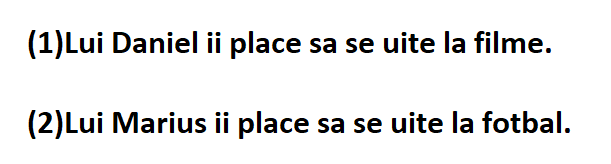
\includegraphics[width=16cm, height=4cm]{figures/cele 2 poze.png}}
			\caption{Propoziții pentru exemplu}
			\label{fig}
		\end{figure}
\par După ce scoatem cuvintele de legătură: lui, îi, să, se, prima propoziție va arată Daniel, place, uite, filme , iar a două Marius place uite fotbal. După ce se lipesc cele două propoziții câmpul cuvintelor va fi: Daniel, place, uite, filme, Marius, fotbal. Apoi vectori care se vor creea pentru cele două propoziții vor arată în felul următor: 

		\begin{figure}[htbp]
			\centerline{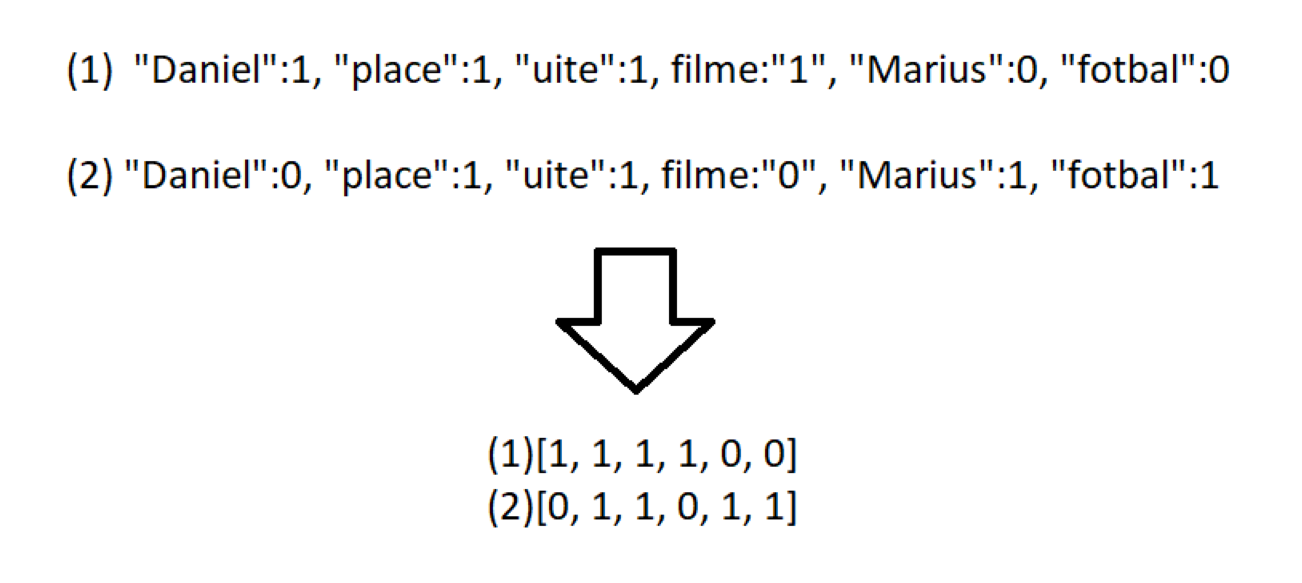
\includegraphics[width=16cm, height=9cm]{figures/rezultat vectori.png}}
			\caption{Propoziții pentru exemplu}
			\label{fig}
		\end{figure}

\section{Similaritatea cosinus }
\par Matricea de similaritate cosinus este utilizată pentru a determina cât de asemănătoare sunt documentele, indiferent de mărimea lor. Aceasta estimează matematic cosinusul unghiului format de doi vectori proiectați într-un spațiu multidimensional. Similaritatea cosinusului este utilă deoarece, chiar dacă două documente comparabile sunt separate de o distanță euclidiană mare (din cauza dimensiunii documentelor), este probabil că acestea să fie similare. Pentru acest model, se folosește similaritatea cosinusului pentru a defini "similitudinea" dintre filme. Motivul pentru care nu se folosește doar distanța dintre vectori ca scor de similaritate, chiar dacă ar putea părea rezonabil, lungimile vectorilor pot afecta distanța euclidiană, dar nu și distanța cosinus (1 - cos(unghi)). Deoarece lungimile a doi vectori definesc dimensiunea acestora (de exemplu, cantitatea de date), dar unghiul definește mai bine caracteristicile lor în lipsa unor cuvinte mai bune. Prin urmare, distanța unghiulară este mai potrivită pentru a defini similitudinea lor.
		\begin{figure}[htbp]
			\centerline{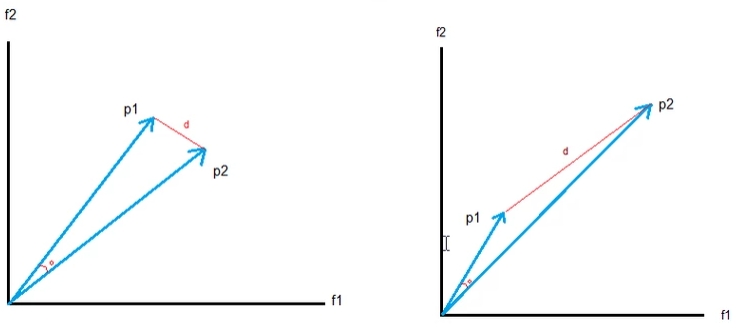
\includegraphics[width=12cm, height=5cm]{figures/grafic distanta.png}}
			\caption{Distanța euclidiană vs. distanța unghiulară}
			\label{fig}
		\end{figure}
\par După cum se poate  vedea, distanța euclidiană devine mult mai mare pe al doilea grafic, chiar dacă unghiul este destul de mic.

\section{Calcularea scorului final}
\par După ce se calculează o matrice în care perechea (i,j) reprezintă similaritatea cosinus dintre două filme se calculează încă o matrice care va reprezenta scorul final. Similaritatea cosinus va fi îmbunătățită în funcție de cât de apreciat este un film astfel rating-ul general a unui film va face diferenta dintre filme cu similaritate apropiata fiind adaugat la scoru matricea de similaritati o valoare in functie de rating. La final se vor lua cele mai mari n scoruri , n reprezentând numărul de filme pe care vrem să le recomandăm, exceptându-l pe primul deoarece cel mai bun scor îl va avea filmul însuși.